\documentclass[twoside]{book}

% Packages required by doxygen
\usepackage{fixltx2e}
\usepackage{calc}
\usepackage{doxygen}
\usepackage[export]{adjustbox} % also loads graphicx
\usepackage{graphicx}
\usepackage[utf8]{inputenc}
\usepackage{makeidx}
\usepackage{multicol}
\usepackage{multirow}
\PassOptionsToPackage{warn}{textcomp}
\usepackage{textcomp}
\usepackage[nointegrals]{wasysym}
\usepackage[table]{xcolor}

% Font selection
\usepackage[T1]{fontenc}
\usepackage[scaled=.90]{helvet}
\usepackage{courier}
\usepackage{amssymb}
\usepackage{sectsty}
\renewcommand{\familydefault}{\sfdefault}
\allsectionsfont{%
  \fontseries{bc}\selectfont%
  \color{darkgray}%
}
\renewcommand{\DoxyLabelFont}{%
  \fontseries{bc}\selectfont%
  \color{darkgray}%
}
\newcommand{\+}{\discretionary{\mbox{\scriptsize$\hookleftarrow$}}{}{}}

% Page & text layout
\usepackage{geometry}
\geometry{%
  a4paper,%
  top=2.5cm,%
  bottom=2.5cm,%
  left=2.5cm,%
  right=2.5cm%
}
\tolerance=750
\hfuzz=15pt
\hbadness=750
\setlength{\emergencystretch}{15pt}
\setlength{\parindent}{0cm}
\setlength{\parskip}{0.2cm}
\makeatletter
\renewcommand{\paragraph}{%
  \@startsection{paragraph}{4}{0ex}{-1.0ex}{1.0ex}{%
    \normalfont\normalsize\bfseries\SS@parafont%
  }%
}
\renewcommand{\subparagraph}{%
  \@startsection{subparagraph}{5}{0ex}{-1.0ex}{1.0ex}{%
    \normalfont\normalsize\bfseries\SS@subparafont%
  }%
}
\makeatother

% Headers & footers
\usepackage{fancyhdr}
\pagestyle{fancyplain}
\fancyhead[LE]{\fancyplain{}{\bfseries\thepage}}
\fancyhead[CE]{\fancyplain{}{}}
\fancyhead[RE]{\fancyplain{}{\bfseries\leftmark}}
\fancyhead[LO]{\fancyplain{}{\bfseries\rightmark}}
\fancyhead[CO]{\fancyplain{}{}}
\fancyhead[RO]{\fancyplain{}{\bfseries\thepage}}
\fancyfoot[LE]{\fancyplain{}{}}
\fancyfoot[CE]{\fancyplain{}{}}
\fancyfoot[RE]{\fancyplain{}{\bfseries\scriptsize Generated on Sun Jan 31 2016 16\+:32\+:25 for Labb1a by Doxygen }}
\fancyfoot[LO]{\fancyplain{}{\bfseries\scriptsize Generated on Sun Jan 31 2016 16\+:32\+:25 for Labb1a by Doxygen }}
\fancyfoot[CO]{\fancyplain{}{}}
\fancyfoot[RO]{\fancyplain{}{}}
\renewcommand{\footrulewidth}{0.4pt}
\renewcommand{\chaptermark}[1]{%
  \markboth{#1}{}%
}
\renewcommand{\sectionmark}[1]{%
  \markright{\thesection\ #1}%
}

% Indices & bibliography
\usepackage{natbib}
\usepackage[titles]{tocloft}
\setcounter{tocdepth}{3}
\setcounter{secnumdepth}{5}
\makeindex

% Hyperlinks (required, but should be loaded last)
\usepackage{ifpdf}
\ifpdf
  \usepackage[pdftex,pagebackref=true]{hyperref}
\else
  \usepackage[ps2pdf,pagebackref=true]{hyperref}
\fi
\hypersetup{%
  colorlinks=true,%
  linkcolor=blue,%
  citecolor=blue,%
  unicode%
}

% Custom commands
\newcommand{\clearemptydoublepage}{%
  \newpage{\pagestyle{empty}\cleardoublepage}%
}


%===== C O N T E N T S =====

\begin{document}

% Titlepage & ToC
\hypersetup{pageanchor=false,
             bookmarks=true,
             bookmarksnumbered=true,
             pdfencoding=unicode
            }
\pagenumbering{roman}
\begin{titlepage}
\vspace*{7cm}
\begin{center}%
{\Large Labb1a }\\
\vspace*{1cm}
{\large Generated by Doxygen 1.8.9.1}\\
\vspace*{0.5cm}
{\small Sun Jan 31 2016 16:32:25}\\
\end{center}
\end{titlepage}
\clearemptydoublepage
\tableofcontents
\clearemptydoublepage
\pagenumbering{arabic}
\hypersetup{pageanchor=true}

%--- Begin generated contents ---
\chapter{Hierarchical Index}
\section{Class Hierarchy}
This inheritance list is sorted roughly, but not completely, alphabetically\+:\begin{DoxyCompactList}
\item \contentsline{section}{Entity}{\pageref{class_entity}}{}
\begin{DoxyCompactList}
\item \contentsline{section}{Workers}{\pageref{class_workers}}{}
\end{DoxyCompactList}
\item \contentsline{section}{Entity\+Manager}{\pageref{class_entity_manager}}{}
\item \contentsline{section}{Message\+Dispatcher}{\pageref{class_message_dispatcher}}{}
\item \contentsline{section}{State$<$ entity\+\_\+type $>$}{\pageref{class_state}}{}
\item \contentsline{section}{State$<$ Workers $>$}{\pageref{class_state}}{}
\begin{DoxyCompactList}
\item \contentsline{section}{Eat\+At\+Bar}{\pageref{class_eat_at_bar}}{}
\item \contentsline{section}{Entity\+Dead}{\pageref{class_entity_dead}}{}
\item \contentsline{section}{Go\+Fishing}{\pageref{class_go_fishing}}{}
\item \contentsline{section}{Go\+Home}{\pageref{class_go_home}}{}
\item \contentsline{section}{Go\+Logging}{\pageref{class_go_logging}}{}
\item \contentsline{section}{Go\+Mining}{\pageref{class_go_mining}}{}
\item \contentsline{section}{Go\+To\+Market}{\pageref{class_go_to_market}}{}
\item \contentsline{section}{Go\+To\+Well}{\pageref{class_go_to_well}}{}
\item \contentsline{section}{Work\+At\+Market}{\pageref{class_work_at_market}}{}
\end{DoxyCompactList}
\item \contentsline{section}{State\+Machine$<$ entity\+\_\+type $>$}{\pageref{class_state_machine}}{}
\item \contentsline{section}{State\+Machine$<$ Workers $>$}{\pageref{class_state_machine}}{}
\item \contentsline{section}{Telegram}{\pageref{struct_telegram}}{}
\end{DoxyCompactList}

\chapter{Class Index}
\section{Class List}
Here are the classes, structs, unions and interfaces with brief descriptions\+:\begin{DoxyCompactList}
\item\contentsline{section}{\hyperlink{class_eat_at_bar}{Eat\+At\+Bar} }{\pageref{class_eat_at_bar}}{}
\item\contentsline{section}{\hyperlink{class_entity}{Entity} }{\pageref{class_entity}}{}
\item\contentsline{section}{\hyperlink{class_entity_dead}{Entity\+Dead} }{\pageref{class_entity_dead}}{}
\item\contentsline{section}{\hyperlink{class_entity_manager}{Entity\+Manager} }{\pageref{class_entity_manager}}{}
\item\contentsline{section}{\hyperlink{class_go_fishing}{Go\+Fishing} }{\pageref{class_go_fishing}}{}
\item\contentsline{section}{\hyperlink{class_go_home}{Go\+Home} }{\pageref{class_go_home}}{}
\item\contentsline{section}{\hyperlink{class_go_logging}{Go\+Logging} }{\pageref{class_go_logging}}{}
\item\contentsline{section}{\hyperlink{class_go_mining}{Go\+Mining} }{\pageref{class_go_mining}}{}
\item\contentsline{section}{\hyperlink{class_go_to_market}{Go\+To\+Market} }{\pageref{class_go_to_market}}{}
\item\contentsline{section}{\hyperlink{class_go_to_well}{Go\+To\+Well} }{\pageref{class_go_to_well}}{}
\item\contentsline{section}{\hyperlink{class_message_dispatcher}{Message\+Dispatcher} }{\pageref{class_message_dispatcher}}{}
\item\contentsline{section}{\hyperlink{class_state}{State$<$ entity\+\_\+type $>$} }{\pageref{class_state}}{}
\item\contentsline{section}{\hyperlink{class_state_machine}{State\+Machine$<$ entity\+\_\+type $>$} }{\pageref{class_state_machine}}{}
\item\contentsline{section}{\hyperlink{struct_telegram}{Telegram} }{\pageref{struct_telegram}}{}
\item\contentsline{section}{\hyperlink{class_work_at_market}{Work\+At\+Market} }{\pageref{class_work_at_market}}{}
\item\contentsline{section}{\hyperlink{class_workers}{Workers} }{\pageref{class_workers}}{}
\end{DoxyCompactList}

\chapter{Class Documentation}
\hypertarget{class_eat_at_bar}{}\section{Eat\+At\+Bar Class Reference}
\label{class_eat_at_bar}\index{Eat\+At\+Bar@{Eat\+At\+Bar}}
Inheritance diagram for Eat\+At\+Bar\+:\begin{figure}[H]
\begin{center}
\leavevmode
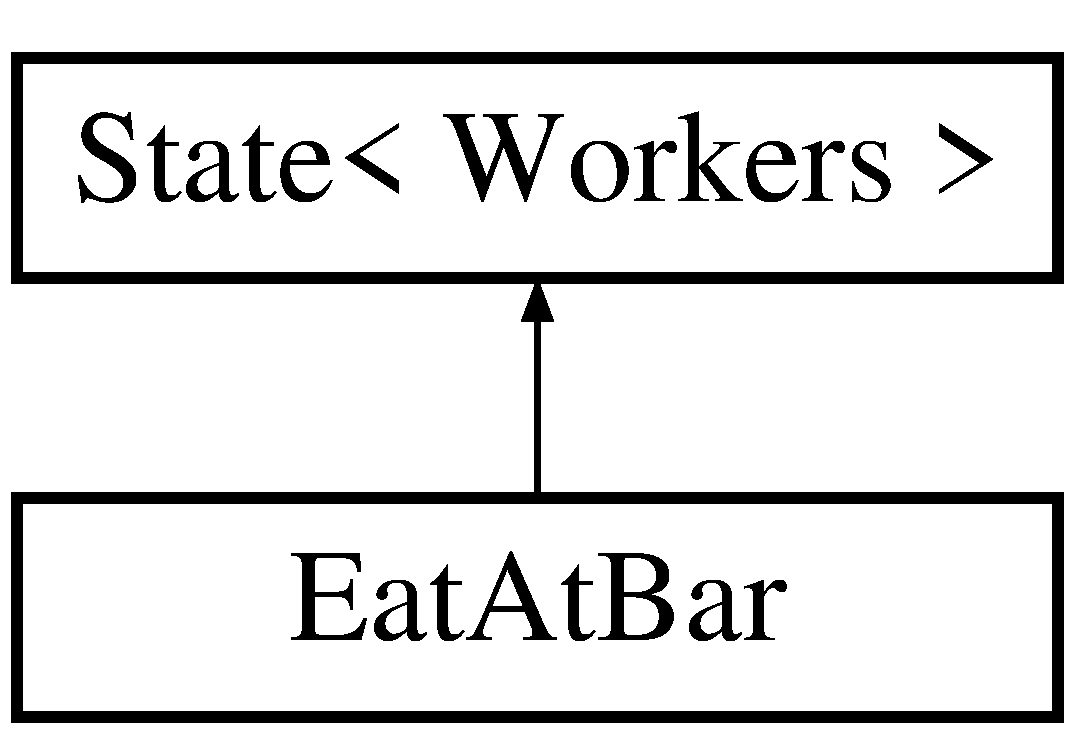
\includegraphics[height=2.000000cm]{class_eat_at_bar}
\end{center}
\end{figure}
\subsection*{Public Member Functions}
\begin{DoxyCompactItemize}
\item 
\hypertarget{class_eat_at_bar_ad05d58b203450c21976326eb1a54ce07}{}virtual void {\bfseries State\+Enter} (\hyperlink{class_workers}{Workers} $\ast$worker)\label{class_eat_at_bar_ad05d58b203450c21976326eb1a54ce07}

\item 
\hypertarget{class_eat_at_bar_ab49293e714036c86c1e1945d3ca8cdce}{}virtual void {\bfseries Execute} (\hyperlink{class_workers}{Workers} $\ast$worker)\label{class_eat_at_bar_ab49293e714036c86c1e1945d3ca8cdce}

\item 
\hypertarget{class_eat_at_bar_ad7d3e2d4a470e785643803691f57cf71}{}virtual void {\bfseries State\+Exit} (\hyperlink{class_workers}{Workers} $\ast$worker)\label{class_eat_at_bar_ad7d3e2d4a470e785643803691f57cf71}

\item 
\hypertarget{class_eat_at_bar_a9a63824bb51ef611a7ed95f21e917739}{}bool {\bfseries On\+Message} (\hyperlink{class_workers}{Workers} $\ast$worker, const \hyperlink{struct_telegram}{Telegram} \&msg)\label{class_eat_at_bar_a9a63824bb51ef611a7ed95f21e917739}

\end{DoxyCompactItemize}
\subsection*{Static Public Member Functions}
\begin{DoxyCompactItemize}
\item 
\hypertarget{class_eat_at_bar_a126d5fbc290f152f4b10d1dea88623af}{}static \hyperlink{class_eat_at_bar}{Eat\+At\+Bar} $\ast$ {\bfseries Instance} ()\label{class_eat_at_bar_a126d5fbc290f152f4b10d1dea88623af}

\end{DoxyCompactItemize}


The documentation for this class was generated from the following files\+:\begin{DoxyCompactItemize}
\item 
Labb1a/Entity\+States.\+h\item 
Labb1a/Entity\+States.\+cpp\end{DoxyCompactItemize}

\hypertarget{class_entity}{}\section{Entity Class Reference}
\label{class_entity}\index{Entity@{Entity}}
Inheritance diagram for Entity\+:\begin{figure}[H]
\begin{center}
\leavevmode
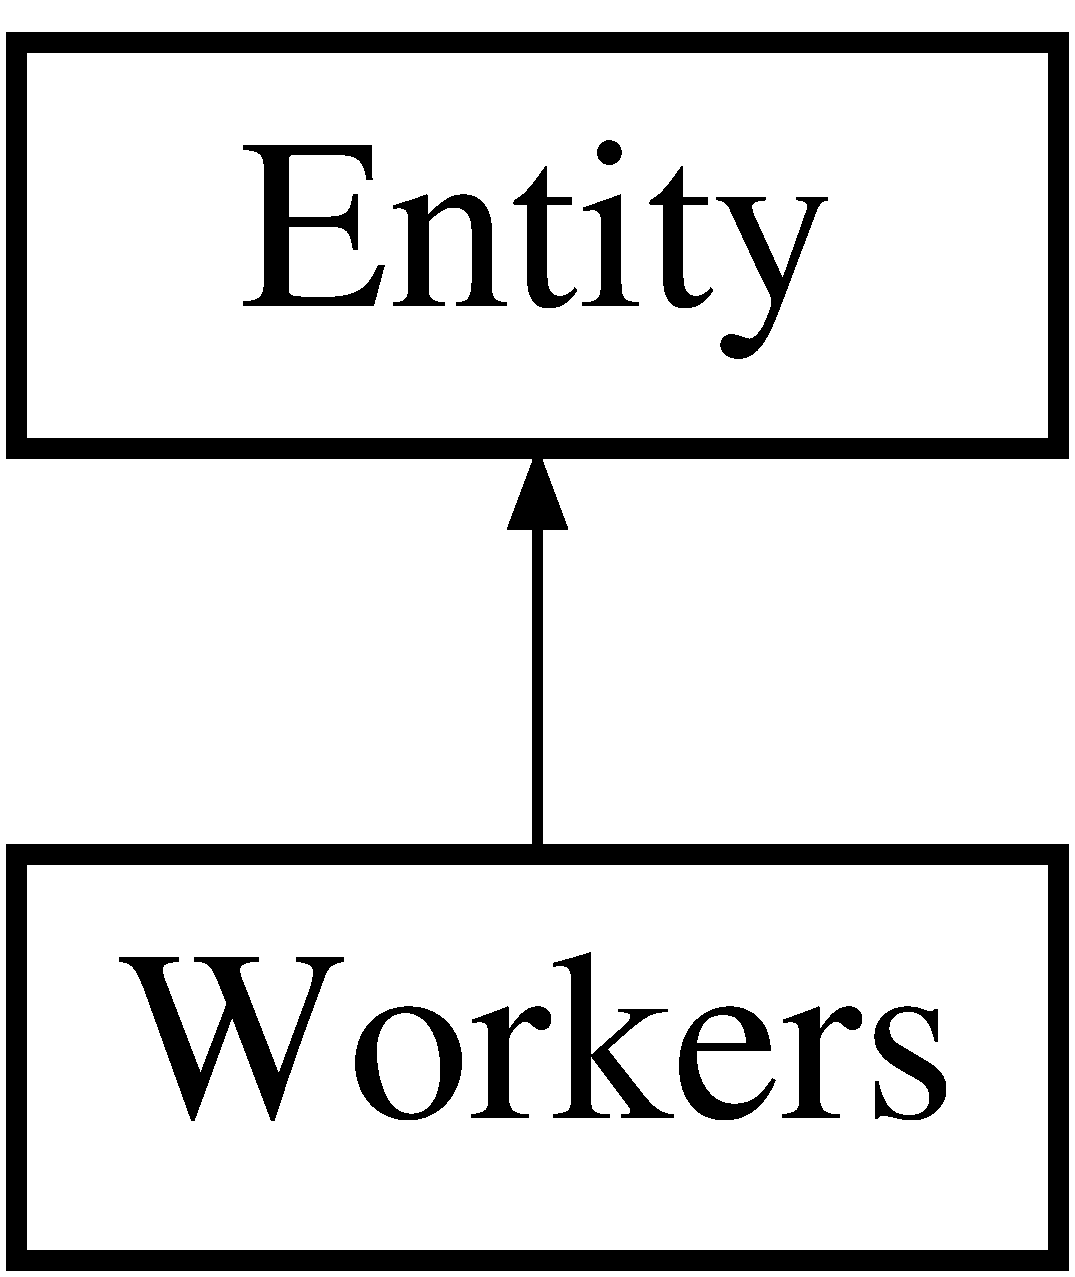
\includegraphics[height=2.000000cm]{class_entity}
\end{center}
\end{figure}
\subsection*{Public Member Functions}
\begin{DoxyCompactItemize}
\item 
\hypertarget{class_entity_ac98bd610e0299cc2aa0538fb2884ab69}{}{\bfseries Entity} (int id)\label{class_entity_ac98bd610e0299cc2aa0538fb2884ab69}

\item 
\hypertarget{class_entity_aa9ee05393626060907a710597103ad43}{}virtual void {\bfseries Update} ()=0\label{class_entity_aa9ee05393626060907a710597103ad43}

\item 
\hypertarget{class_entity_a3c60d3c0561843490e93bde1f4566900}{}int {\bfseries get\+I\+D} ()\label{class_entity_a3c60d3c0561843490e93bde1f4566900}

\item 
\hypertarget{class_entity_acfbd9622ebb9948cf4bc3700b04ab75a}{}virtual bool {\bfseries Handle\+Message} (const \hyperlink{struct_telegram}{Telegram} \&msg)=0\label{class_entity_acfbd9622ebb9948cf4bc3700b04ab75a}

\item 
\hypertarget{class_entity_ab27dd18ecddf029d24c73ef076409f42}{}virtual location\+\_\+type {\bfseries get\+Location} ()=0\label{class_entity_ab27dd18ecddf029d24c73ef076409f42}

\end{DoxyCompactItemize}


The documentation for this class was generated from the following files\+:\begin{DoxyCompactItemize}
\item 
Labb1a/Entity.\+h\item 
Labb1a/Entity.\+cpp\end{DoxyCompactItemize}

\hypertarget{class_entity_dead}{}\section{Entity\+Dead Class Reference}
\label{class_entity_dead}\index{Entity\+Dead@{Entity\+Dead}}
Inheritance diagram for Entity\+Dead\+:\begin{figure}[H]
\begin{center}
\leavevmode
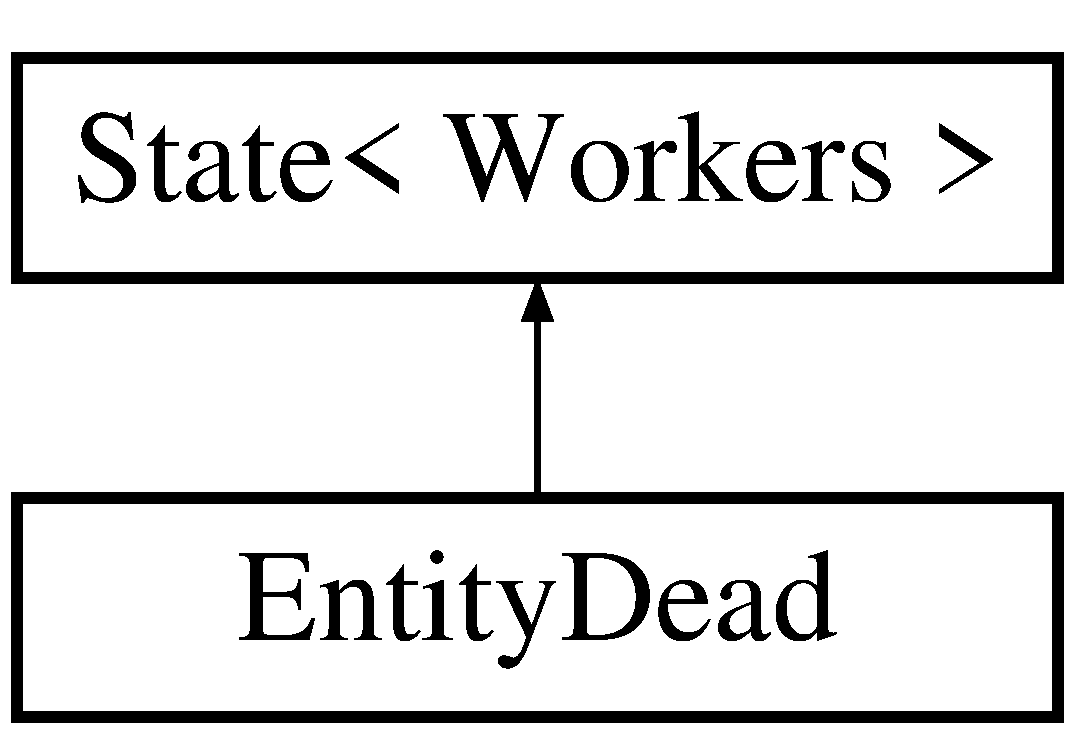
\includegraphics[height=2.000000cm]{class_entity_dead}
\end{center}
\end{figure}
\subsection*{Public Member Functions}
\begin{DoxyCompactItemize}
\item 
\hypertarget{class_entity_dead_a8591fb80ef0fda85b69ed30daf0c87ea}{}virtual void {\bfseries State\+Enter} (\hyperlink{class_workers}{Workers} $\ast$worker)\label{class_entity_dead_a8591fb80ef0fda85b69ed30daf0c87ea}

\item 
\hypertarget{class_entity_dead_a9268fe0bece256533c88e1d3dfefb992}{}virtual void {\bfseries Execute} (\hyperlink{class_workers}{Workers} $\ast$worker)\label{class_entity_dead_a9268fe0bece256533c88e1d3dfefb992}

\item 
\hypertarget{class_entity_dead_a29c8d2b1e807d82cea45e540b5d88fc1}{}virtual void {\bfseries State\+Exit} (\hyperlink{class_workers}{Workers} $\ast$worker)\label{class_entity_dead_a29c8d2b1e807d82cea45e540b5d88fc1}

\item 
\hypertarget{class_entity_dead_aca94d2ec768f14f92df6111fabd19277}{}bool {\bfseries On\+Message} (\hyperlink{class_workers}{Workers} $\ast$worker, const \hyperlink{struct_telegram}{Telegram} \&msg)\label{class_entity_dead_aca94d2ec768f14f92df6111fabd19277}

\end{DoxyCompactItemize}
\subsection*{Static Public Member Functions}
\begin{DoxyCompactItemize}
\item 
\hypertarget{class_entity_dead_aabb45af19bdee64336b4e6be98677303}{}static \hyperlink{class_entity_dead}{Entity\+Dead} $\ast$ {\bfseries Instance} ()\label{class_entity_dead_aabb45af19bdee64336b4e6be98677303}

\end{DoxyCompactItemize}


The documentation for this class was generated from the following files\+:\begin{DoxyCompactItemize}
\item 
Labb1a/Entity\+States.\+h\item 
Labb1a/Entity\+States.\+cpp\end{DoxyCompactItemize}

\hypertarget{class_entity_manager}{}\section{Entity\+Manager Class Reference}
\label{class_entity_manager}\index{Entity\+Manager@{Entity\+Manager}}
\subsection*{Public Member Functions}
\begin{DoxyCompactItemize}
\item 
\hypertarget{class_entity_manager_a5ada06752ff17e52487c40253b9807ac}{}void {\bfseries Register\+Entity} (\hyperlink{class_entity}{Entity} $\ast$new\+Ent)\label{class_entity_manager_a5ada06752ff17e52487c40253b9807ac}

\item 
\hypertarget{class_entity_manager_a62c851c5f750c5d88d761eeb6c3757c2}{}\hyperlink{class_entity}{Entity} $\ast$ {\bfseries Get\+Entity} (int id)\label{class_entity_manager_a62c851c5f750c5d88d761eeb6c3757c2}

\item 
\hypertarget{class_entity_manager_ae0ab17f0fa95c0e46f0bb7b96ae7df71}{}void {\bfseries Remove\+Entity} (\hyperlink{class_entity}{Entity} $\ast$ent)\label{class_entity_manager_ae0ab17f0fa95c0e46f0bb7b96ae7df71}

\end{DoxyCompactItemize}
\subsection*{Static Public Member Functions}
\begin{DoxyCompactItemize}
\item 
\hypertarget{class_entity_manager_a8dd5a07092d1c2220c53dfc524e28ef8}{}static \hyperlink{class_entity_manager}{Entity\+Manager} $\ast$ {\bfseries Instance} ()\label{class_entity_manager_a8dd5a07092d1c2220c53dfc524e28ef8}

\end{DoxyCompactItemize}


The documentation for this class was generated from the following files\+:\begin{DoxyCompactItemize}
\item 
Labb1a/Entity\+Manager.\+h\item 
Labb1a/Entity\+Manager.\+cpp\end{DoxyCompactItemize}

\hypertarget{class_go_fishing}{}\section{Go\+Fishing Class Reference}
\label{class_go_fishing}\index{Go\+Fishing@{Go\+Fishing}}
Inheritance diagram for Go\+Fishing\+:\begin{figure}[H]
\begin{center}
\leavevmode
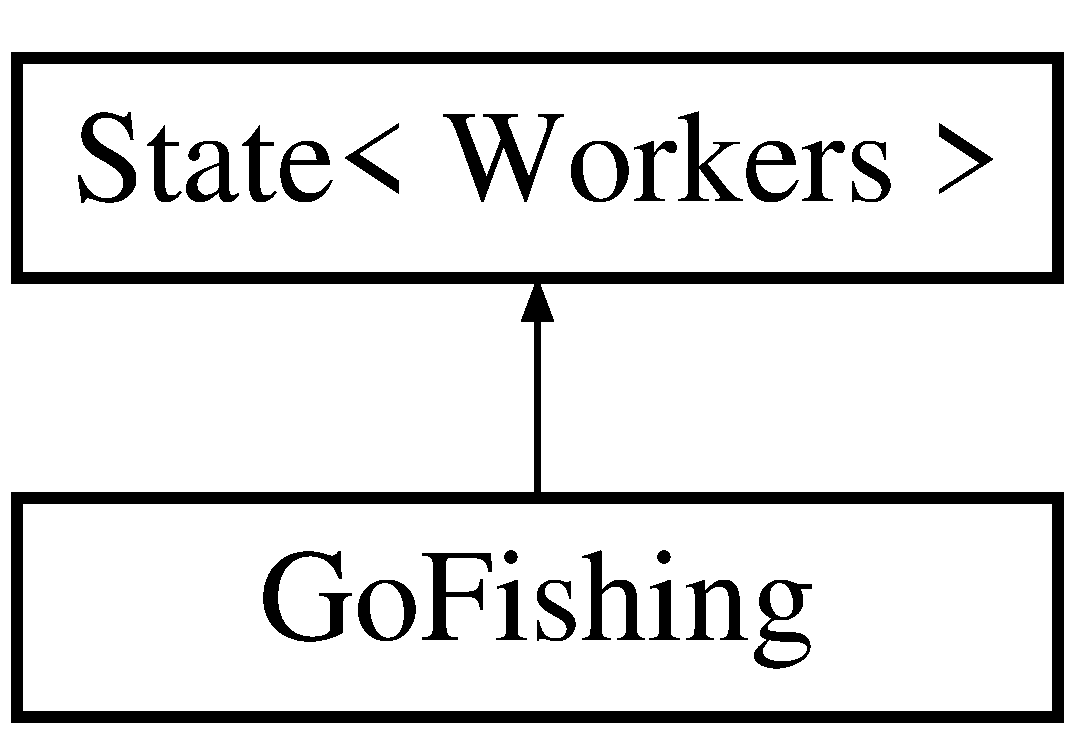
\includegraphics[height=2.000000cm]{class_go_fishing}
\end{center}
\end{figure}
\subsection*{Public Member Functions}
\begin{DoxyCompactItemize}
\item 
\hypertarget{class_go_fishing_a520b14116f317b4ab51f58bd5bd451e1}{}virtual void {\bfseries State\+Enter} (\hyperlink{class_workers}{Workers} $\ast$worker)\label{class_go_fishing_a520b14116f317b4ab51f58bd5bd451e1}

\item 
\hypertarget{class_go_fishing_aaa681dde7d4618c9232b2884b8d14f03}{}virtual void {\bfseries Execute} (\hyperlink{class_workers}{Workers} $\ast$worker)\label{class_go_fishing_aaa681dde7d4618c9232b2884b8d14f03}

\item 
\hypertarget{class_go_fishing_a27ca60ebcd6d2a42b09f75f859f71ea5}{}virtual void {\bfseries State\+Exit} (\hyperlink{class_workers}{Workers} $\ast$worker)\label{class_go_fishing_a27ca60ebcd6d2a42b09f75f859f71ea5}

\item 
\hypertarget{class_go_fishing_abce7a197684866e0c3851eff9d31694a}{}bool {\bfseries On\+Message} (\hyperlink{class_workers}{Workers} $\ast$worker, const \hyperlink{struct_telegram}{Telegram} \&msg)\label{class_go_fishing_abce7a197684866e0c3851eff9d31694a}

\end{DoxyCompactItemize}
\subsection*{Static Public Member Functions}
\begin{DoxyCompactItemize}
\item 
\hypertarget{class_go_fishing_a8309a9bcbf5de86c6e782ab66b088450}{}static \hyperlink{class_go_fishing}{Go\+Fishing} $\ast$ {\bfseries Instance} ()\label{class_go_fishing_a8309a9bcbf5de86c6e782ab66b088450}

\end{DoxyCompactItemize}


The documentation for this class was generated from the following files\+:\begin{DoxyCompactItemize}
\item 
Labb1a/Entity\+States.\+h\item 
Labb1a/Entity\+States.\+cpp\end{DoxyCompactItemize}

\hypertarget{class_go_home}{}\section{Go\+Home Class Reference}
\label{class_go_home}\index{Go\+Home@{Go\+Home}}
Inheritance diagram for Go\+Home\+:\begin{figure}[H]
\begin{center}
\leavevmode
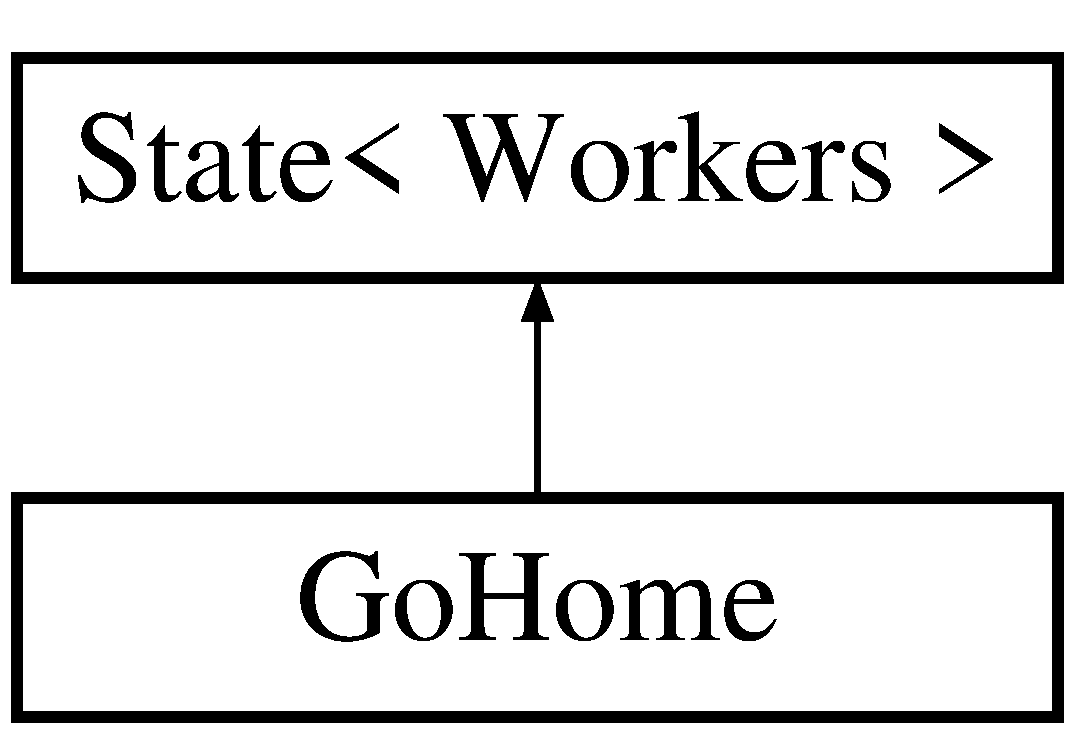
\includegraphics[height=2.000000cm]{class_go_home}
\end{center}
\end{figure}
\subsection*{Public Member Functions}
\begin{DoxyCompactItemize}
\item 
\hypertarget{class_go_home_a82f45f37c4a91ced544ffed1261e3ab8}{}virtual void {\bfseries State\+Enter} (\hyperlink{class_workers}{Workers} $\ast$worker)\label{class_go_home_a82f45f37c4a91ced544ffed1261e3ab8}

\item 
\hypertarget{class_go_home_a19fd88f9340c496e918f4af6e1dbc0e6}{}virtual void {\bfseries Execute} (\hyperlink{class_workers}{Workers} $\ast$worker)\label{class_go_home_a19fd88f9340c496e918f4af6e1dbc0e6}

\item 
\hypertarget{class_go_home_a36c098bc3ed3fe54222d9e45339b6cc0}{}virtual void {\bfseries State\+Exit} (\hyperlink{class_workers}{Workers} $\ast$worker)\label{class_go_home_a36c098bc3ed3fe54222d9e45339b6cc0}

\item 
\hypertarget{class_go_home_a48a6203c9c883bc4bafd72ab6251d107}{}bool {\bfseries On\+Message} (\hyperlink{class_workers}{Workers} $\ast$worker, const \hyperlink{struct_telegram}{Telegram} \&msg)\label{class_go_home_a48a6203c9c883bc4bafd72ab6251d107}

\end{DoxyCompactItemize}
\subsection*{Static Public Member Functions}
\begin{DoxyCompactItemize}
\item 
\hypertarget{class_go_home_a2b19822453e4e81f6b6f057fbdb2ec7d}{}static \hyperlink{class_go_home}{Go\+Home} $\ast$ {\bfseries Instance} ()\label{class_go_home_a2b19822453e4e81f6b6f057fbdb2ec7d}

\end{DoxyCompactItemize}


The documentation for this class was generated from the following files\+:\begin{DoxyCompactItemize}
\item 
Labb1a/Entity\+States.\+h\item 
Labb1a/Entity\+States.\+cpp\end{DoxyCompactItemize}

\hypertarget{class_go_logging}{}\section{Go\+Logging Class Reference}
\label{class_go_logging}\index{Go\+Logging@{Go\+Logging}}
Inheritance diagram for Go\+Logging\+:\begin{figure}[H]
\begin{center}
\leavevmode
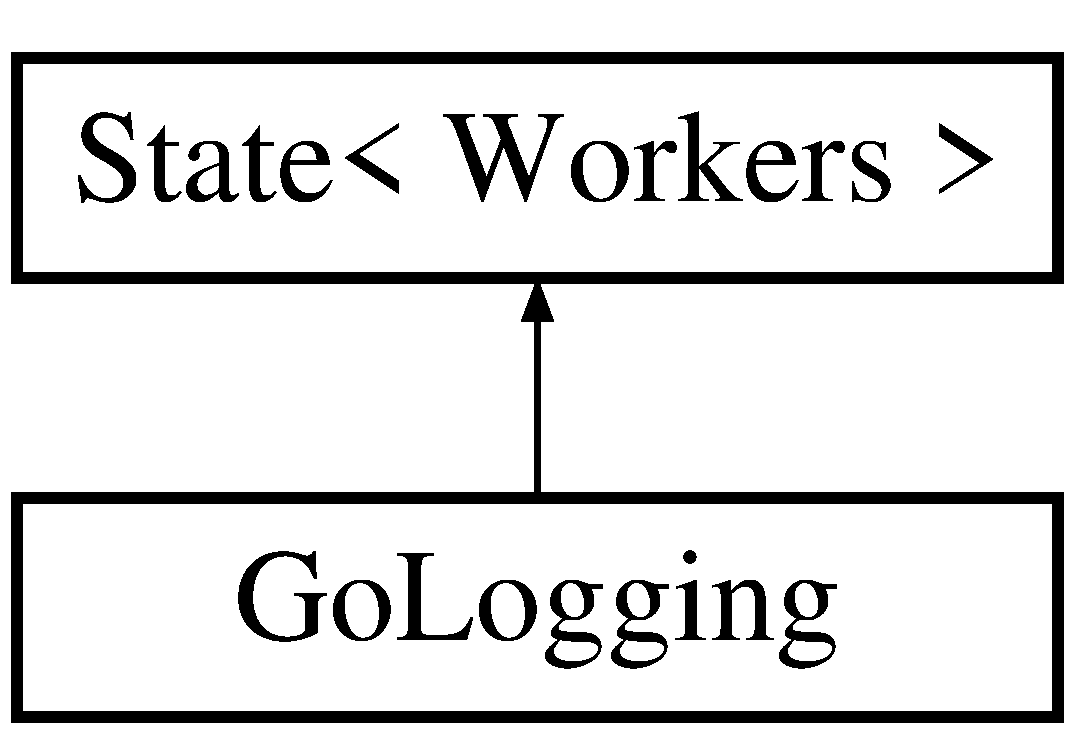
\includegraphics[height=2.000000cm]{class_go_logging}
\end{center}
\end{figure}
\subsection*{Public Member Functions}
\begin{DoxyCompactItemize}
\item 
\hypertarget{class_go_logging_a073579651326fd31ed6a200778bb86f9}{}virtual void {\bfseries State\+Enter} (\hyperlink{class_workers}{Workers} $\ast$worker)\label{class_go_logging_a073579651326fd31ed6a200778bb86f9}

\item 
\hypertarget{class_go_logging_acedd11be0dddff0176fdf91296567af6}{}virtual void {\bfseries Execute} (\hyperlink{class_workers}{Workers} $\ast$worker)\label{class_go_logging_acedd11be0dddff0176fdf91296567af6}

\item 
\hypertarget{class_go_logging_a44a839d51095a5f1266695f9cb6af35c}{}virtual void {\bfseries State\+Exit} (\hyperlink{class_workers}{Workers} $\ast$worker)\label{class_go_logging_a44a839d51095a5f1266695f9cb6af35c}

\item 
\hypertarget{class_go_logging_ac04459d45c836a6d95b01c95011494bc}{}bool {\bfseries On\+Message} (\hyperlink{class_workers}{Workers} $\ast$worker, const \hyperlink{struct_telegram}{Telegram} \&msg)\label{class_go_logging_ac04459d45c836a6d95b01c95011494bc}

\end{DoxyCompactItemize}
\subsection*{Static Public Member Functions}
\begin{DoxyCompactItemize}
\item 
\hypertarget{class_go_logging_a8fd8d4e719045323fc359870e930141d}{}static \hyperlink{class_go_logging}{Go\+Logging} $\ast$ {\bfseries Instance} ()\label{class_go_logging_a8fd8d4e719045323fc359870e930141d}

\end{DoxyCompactItemize}


The documentation for this class was generated from the following files\+:\begin{DoxyCompactItemize}
\item 
Labb1a/Entity\+States.\+h\item 
Labb1a/Entity\+States.\+cpp\end{DoxyCompactItemize}

\hypertarget{class_go_mining}{}\section{Go\+Mining Class Reference}
\label{class_go_mining}\index{Go\+Mining@{Go\+Mining}}
Inheritance diagram for Go\+Mining\+:\begin{figure}[H]
\begin{center}
\leavevmode
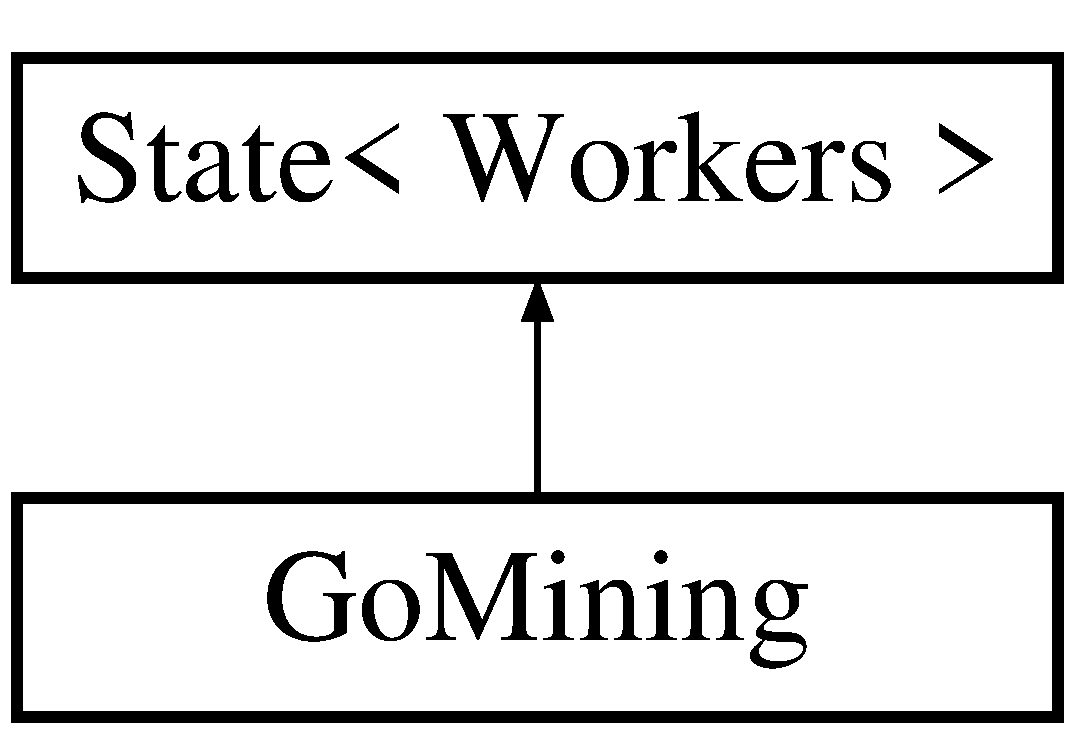
\includegraphics[height=2.000000cm]{class_go_mining}
\end{center}
\end{figure}
\subsection*{Public Member Functions}
\begin{DoxyCompactItemize}
\item 
\hypertarget{class_go_mining_af0b79e9f94e9c8831940b370028ed628}{}virtual void {\bfseries State\+Enter} (\hyperlink{class_workers}{Workers} $\ast$worker)\label{class_go_mining_af0b79e9f94e9c8831940b370028ed628}

\item 
\hypertarget{class_go_mining_a0b6bc0558351394e8f21cdada67e5798}{}virtual void {\bfseries Execute} (\hyperlink{class_workers}{Workers} $\ast$worker)\label{class_go_mining_a0b6bc0558351394e8f21cdada67e5798}

\item 
\hypertarget{class_go_mining_a14a2a824d0b1a2f0f6dcf7cc50caf76d}{}virtual void {\bfseries State\+Exit} (\hyperlink{class_workers}{Workers} $\ast$worker)\label{class_go_mining_a14a2a824d0b1a2f0f6dcf7cc50caf76d}

\item 
\hypertarget{class_go_mining_a1c6d47e453dfc5c75a789a77026a1488}{}bool {\bfseries On\+Message} (\hyperlink{class_workers}{Workers} $\ast$worker, const \hyperlink{struct_telegram}{Telegram} \&msg)\label{class_go_mining_a1c6d47e453dfc5c75a789a77026a1488}

\end{DoxyCompactItemize}
\subsection*{Static Public Member Functions}
\begin{DoxyCompactItemize}
\item 
\hypertarget{class_go_mining_a01ae560d43f2a7970cfa0299051e8870}{}static \hyperlink{class_go_mining}{Go\+Mining} $\ast$ {\bfseries Instance} ()\label{class_go_mining_a01ae560d43f2a7970cfa0299051e8870}

\end{DoxyCompactItemize}


The documentation for this class was generated from the following files\+:\begin{DoxyCompactItemize}
\item 
Labb1a/Entity\+States.\+h\item 
Labb1a/Entity\+States.\+cpp\end{DoxyCompactItemize}

\hypertarget{class_go_to_market}{}\section{Go\+To\+Market Class Reference}
\label{class_go_to_market}\index{Go\+To\+Market@{Go\+To\+Market}}
Inheritance diagram for Go\+To\+Market\+:\begin{figure}[H]
\begin{center}
\leavevmode
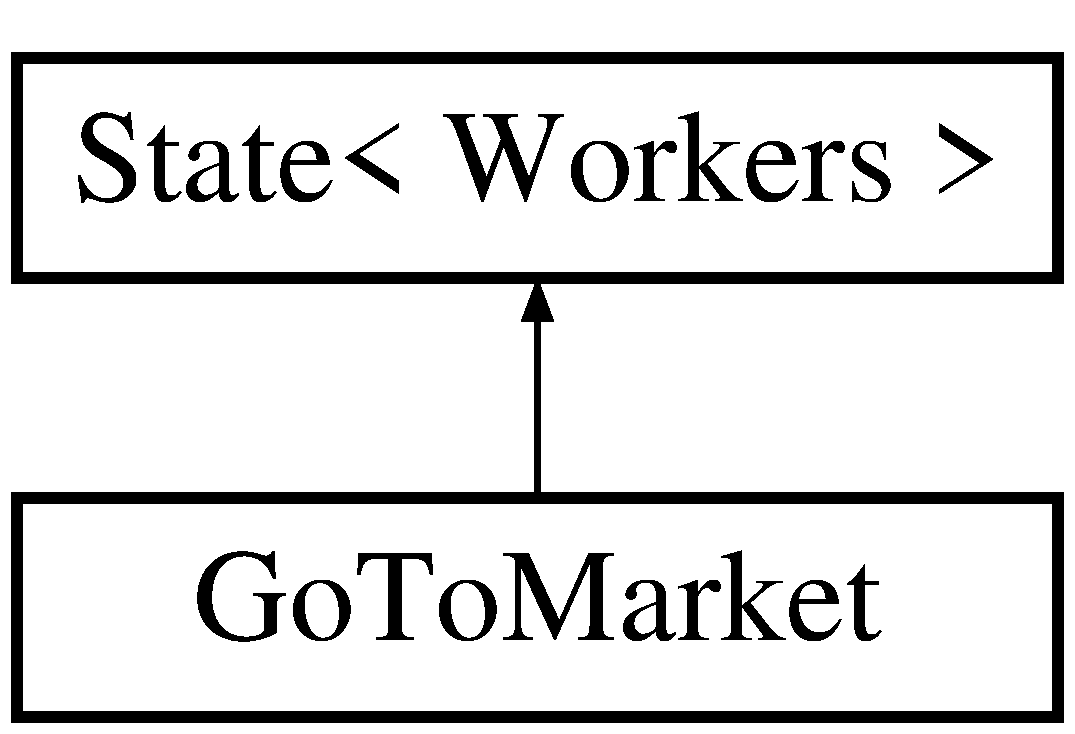
\includegraphics[height=2.000000cm]{class_go_to_market}
\end{center}
\end{figure}
\subsection*{Public Member Functions}
\begin{DoxyCompactItemize}
\item 
\hypertarget{class_go_to_market_a81aa2ce2930ff457c5ff2324f53cacaa}{}virtual void {\bfseries State\+Enter} (\hyperlink{class_workers}{Workers} $\ast$worker)\label{class_go_to_market_a81aa2ce2930ff457c5ff2324f53cacaa}

\item 
\hypertarget{class_go_to_market_a021b364ed9397c216a2dc99920cc19cb}{}virtual void {\bfseries Execute} (\hyperlink{class_workers}{Workers} $\ast$worker)\label{class_go_to_market_a021b364ed9397c216a2dc99920cc19cb}

\item 
\hypertarget{class_go_to_market_a386a2fed19e9c00504ebed3bbd5b8861}{}virtual void {\bfseries State\+Exit} (\hyperlink{class_workers}{Workers} $\ast$worker)\label{class_go_to_market_a386a2fed19e9c00504ebed3bbd5b8861}

\item 
\hypertarget{class_go_to_market_a81632944bc84023345834e24eb0498a2}{}bool {\bfseries On\+Message} (\hyperlink{class_workers}{Workers} $\ast$worker, const \hyperlink{struct_telegram}{Telegram} \&msg)\label{class_go_to_market_a81632944bc84023345834e24eb0498a2}

\end{DoxyCompactItemize}
\subsection*{Static Public Member Functions}
\begin{DoxyCompactItemize}
\item 
\hypertarget{class_go_to_market_ab105de7dc42a8b9a94fd0976995ce319}{}static \hyperlink{class_go_to_market}{Go\+To\+Market} $\ast$ {\bfseries Instance} ()\label{class_go_to_market_ab105de7dc42a8b9a94fd0976995ce319}

\end{DoxyCompactItemize}


The documentation for this class was generated from the following files\+:\begin{DoxyCompactItemize}
\item 
Labb1a/Entity\+States.\+h\item 
Labb1a/Entity\+States.\+cpp\end{DoxyCompactItemize}

\hypertarget{class_go_to_well}{}\section{Go\+To\+Well Class Reference}
\label{class_go_to_well}\index{Go\+To\+Well@{Go\+To\+Well}}
Inheritance diagram for Go\+To\+Well\+:\begin{figure}[H]
\begin{center}
\leavevmode
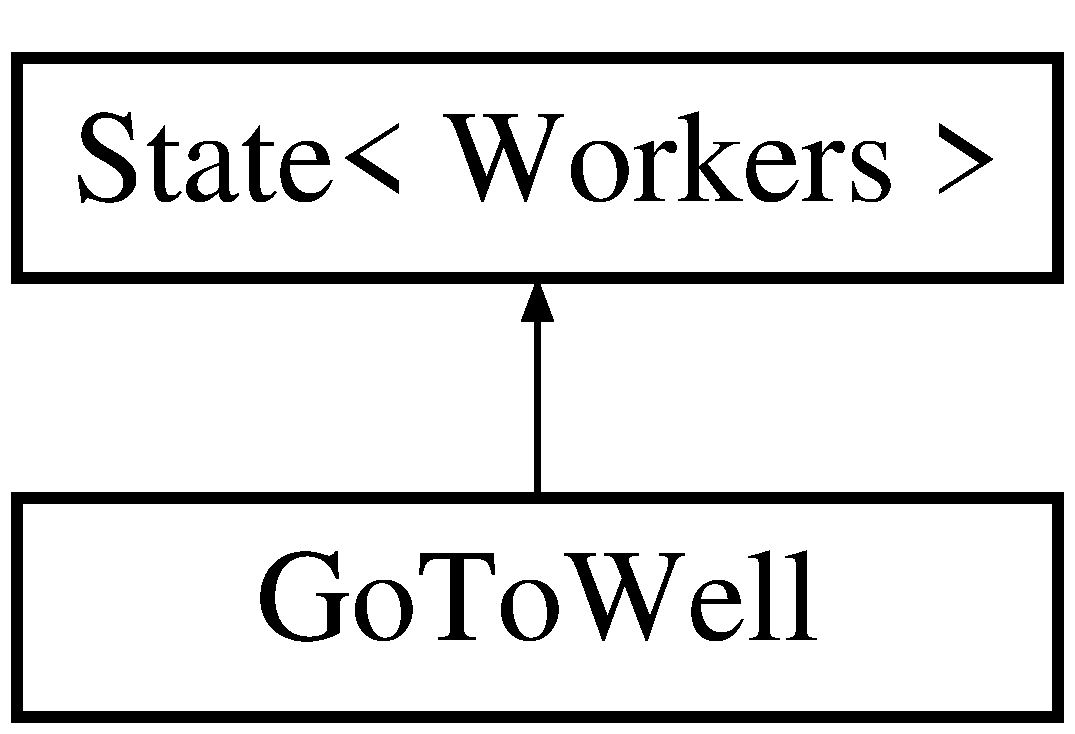
\includegraphics[height=2.000000cm]{class_go_to_well}
\end{center}
\end{figure}
\subsection*{Public Member Functions}
\begin{DoxyCompactItemize}
\item 
\hypertarget{class_go_to_well_ae31941876646a91c2f8633ad31fb17bc}{}virtual void {\bfseries State\+Enter} (\hyperlink{class_workers}{Workers} $\ast$worker)\label{class_go_to_well_ae31941876646a91c2f8633ad31fb17bc}

\item 
\hypertarget{class_go_to_well_ab15f179542a09f574f11ad2bd51adc13}{}virtual void {\bfseries Execute} (\hyperlink{class_workers}{Workers} $\ast$worker)\label{class_go_to_well_ab15f179542a09f574f11ad2bd51adc13}

\item 
\hypertarget{class_go_to_well_a95e9c640e504ee3e8e66ca08ae400962}{}virtual void {\bfseries State\+Exit} (\hyperlink{class_workers}{Workers} $\ast$worker)\label{class_go_to_well_a95e9c640e504ee3e8e66ca08ae400962}

\item 
\hypertarget{class_go_to_well_af224556cb446a38030fab5bf2f9ad4d8}{}bool {\bfseries On\+Message} (\hyperlink{class_workers}{Workers} $\ast$worker, const \hyperlink{struct_telegram}{Telegram} \&msg)\label{class_go_to_well_af224556cb446a38030fab5bf2f9ad4d8}

\end{DoxyCompactItemize}
\subsection*{Static Public Member Functions}
\begin{DoxyCompactItemize}
\item 
\hypertarget{class_go_to_well_a99c5b8a23dbdaeb3c7d6b003fa849d30}{}static \hyperlink{class_go_to_well}{Go\+To\+Well} $\ast$ {\bfseries Instance} ()\label{class_go_to_well_a99c5b8a23dbdaeb3c7d6b003fa849d30}

\end{DoxyCompactItemize}


The documentation for this class was generated from the following files\+:\begin{DoxyCompactItemize}
\item 
Labb1a/Entity\+States.\+h\item 
Labb1a/Entity\+States.\+cpp\end{DoxyCompactItemize}

\hypertarget{class_message_dispatcher}{}\section{Message\+Dispatcher Class Reference}
\label{class_message_dispatcher}\index{Message\+Dispatcher@{Message\+Dispatcher}}
\subsection*{Public Member Functions}
\begin{DoxyCompactItemize}
\item 
\hypertarget{class_message_dispatcher_a0a206b3af513b20f33bbcfad28e977cb}{}void {\bfseries Dispatch\+Message} (double delay, int sender, int receiver, int msg, void $\ast$extra\+Info)\label{class_message_dispatcher_a0a206b3af513b20f33bbcfad28e977cb}

\end{DoxyCompactItemize}
\subsection*{Static Public Member Functions}
\begin{DoxyCompactItemize}
\item 
\hypertarget{class_message_dispatcher_a8b3571dd8cac14ac0c7695e9904b00c3}{}static \hyperlink{class_message_dispatcher}{Message\+Dispatcher} $\ast$ {\bfseries Instance} ()\label{class_message_dispatcher_a8b3571dd8cac14ac0c7695e9904b00c3}

\end{DoxyCompactItemize}


The documentation for this class was generated from the following files\+:\begin{DoxyCompactItemize}
\item 
Labb1a/Message\+Dispatcher.\+h\item 
Labb1a/Message\+Dispatcher.\+cpp\end{DoxyCompactItemize}

\hypertarget{class_state}{}\section{State$<$ entity\+\_\+type $>$ Class Template Reference}
\label{class_state}\index{State$<$ entity\+\_\+type $>$@{State$<$ entity\+\_\+type $>$}}
\subsection*{Public Member Functions}
\begin{DoxyCompactItemize}
\item 
\hypertarget{class_state_a1c2dad408fca149fc9d8f8dd62c5af1f}{}virtual void {\bfseries State\+Enter} (entity\+\_\+type $\ast$worker)=0\label{class_state_a1c2dad408fca149fc9d8f8dd62c5af1f}

\item 
\hypertarget{class_state_afbc08bc5a96c16658ab00e22cc5e4ef3}{}virtual void {\bfseries Execute} (entity\+\_\+type $\ast$worker)=0\label{class_state_afbc08bc5a96c16658ab00e22cc5e4ef3}

\item 
\hypertarget{class_state_afaedc91ca20b78d3ef2774db4020ff89}{}virtual void {\bfseries State\+Exit} (entity\+\_\+type $\ast$worker)=0\label{class_state_afaedc91ca20b78d3ef2774db4020ff89}

\item 
\hypertarget{class_state_adf18af1793d77f8a0f72e9c92a056d6e}{}virtual bool {\bfseries On\+Message} (entity\+\_\+type $\ast$worker, const \hyperlink{struct_telegram}{Telegram} \&tele)=0\label{class_state_adf18af1793d77f8a0f72e9c92a056d6e}

\end{DoxyCompactItemize}


The documentation for this class was generated from the following file\+:\begin{DoxyCompactItemize}
\item 
Labb1a/State.\+h\end{DoxyCompactItemize}

\hypertarget{class_state_machine}{}\section{State\+Machine$<$ entity\+\_\+type $>$ Class Template Reference}
\label{class_state_machine}\index{State\+Machine$<$ entity\+\_\+type $>$@{State\+Machine$<$ entity\+\_\+type $>$}}
\subsection*{Public Member Functions}
\begin{DoxyCompactItemize}
\item 
\hypertarget{class_state_machine_a336270462a6e76ccbbeab7c3b2f7e23d}{}{\bfseries State\+Machine} (entity\+\_\+type $\ast$p\+Owner)\label{class_state_machine_a336270462a6e76ccbbeab7c3b2f7e23d}

\item 
\hypertarget{class_state_machine_ad09b9f4653c64557ef6d9dc0e306928d}{}void {\bfseries set\+Current\+State} (\hyperlink{class_state}{State}$<$ entity\+\_\+type $>$ $\ast$val)\label{class_state_machine_ad09b9f4653c64557ef6d9dc0e306928d}

\item 
\hypertarget{class_state_machine_aee89a494cfe89298ae6d2501e01311f2}{}void {\bfseries set\+Previous\+State} (\hyperlink{class_state}{State}$<$ entity\+\_\+type $>$ $\ast$val)\label{class_state_machine_aee89a494cfe89298ae6d2501e01311f2}

\item 
\hypertarget{class_state_machine_ad43d3a3bdfc80782ae70b4733f47062c}{}void {\bfseries set\+Global\+State} (\hyperlink{class_state}{State}$<$ entity\+\_\+type $>$ $\ast$val)\label{class_state_machine_ad43d3a3bdfc80782ae70b4733f47062c}

\item 
\hypertarget{class_state_machine_a518dfc4310fad8d96e27a716207dbceb}{}\hyperlink{class_state}{State}$<$ entity\+\_\+type $>$ $\ast$ {\bfseries get\+Current\+State} () const \label{class_state_machine_a518dfc4310fad8d96e27a716207dbceb}

\item 
\hypertarget{class_state_machine_ad6e2eeeb9c91ef21508c80cd9db10f59}{}\hyperlink{class_state}{State}$<$ entity\+\_\+type $>$ $\ast$ {\bfseries get\+Previous\+State} () const \label{class_state_machine_ad6e2eeeb9c91ef21508c80cd9db10f59}

\item 
\hypertarget{class_state_machine_a5067c97c56b065e3e52ba8b8e3ed989c}{}\hyperlink{class_state}{State}$<$ entity\+\_\+type $>$ $\ast$ {\bfseries get\+Global\+State} () const \label{class_state_machine_a5067c97c56b065e3e52ba8b8e3ed989c}

\item 
\hypertarget{class_state_machine_a24b1f38171537058ab8040b3b42adb6c}{}void {\bfseries Update} () const \label{class_state_machine_a24b1f38171537058ab8040b3b42adb6c}

\item 
\hypertarget{class_state_machine_a916699645fd8deb8f0d757825d300d01}{}void {\bfseries Change\+State} (\hyperlink{class_state}{State}$<$ entity\+\_\+type $>$ $\ast$new\+State)\label{class_state_machine_a916699645fd8deb8f0d757825d300d01}

\item 
\hypertarget{class_state_machine_ac75b55d8ea42733057cca0775902324c}{}void {\bfseries Change\+State\+Not\+Working} (\hyperlink{class_state}{State}$<$ entity\+\_\+type $>$ $\ast$new\+State)\label{class_state_machine_ac75b55d8ea42733057cca0775902324c}

\item 
\hypertarget{class_state_machine_ab663cdc952a9ab03417d9ea79badbe92}{}void {\bfseries Revert\+To\+Previous} ()\label{class_state_machine_ab663cdc952a9ab03417d9ea79badbe92}

\item 
\hypertarget{class_state_machine_ab88d69e6b08a87ff14ad1e8e4440d8d4}{}bool {\bfseries is\+In\+State} (const \hyperlink{class_state}{State}$<$ entity\+\_\+type $>$ \&st)\label{class_state_machine_ab88d69e6b08a87ff14ad1e8e4440d8d4}

\item 
\hypertarget{class_state_machine_a657e50b3d54a1f93abc40978be52ea40}{}bool {\bfseries Handle\+Message} (const \hyperlink{struct_telegram}{Telegram} \&msg)\label{class_state_machine_a657e50b3d54a1f93abc40978be52ea40}

\end{DoxyCompactItemize}


The documentation for this class was generated from the following file\+:\begin{DoxyCompactItemize}
\item 
Labb1a/State\+Machine.\+h\end{DoxyCompactItemize}

\hypertarget{struct_telegram}{}\section{Telegram Struct Reference}
\label{struct_telegram}\index{Telegram@{Telegram}}
\subsection*{Public Member Functions}
\begin{DoxyCompactItemize}
\item 
\hypertarget{struct_telegram_a43b0eab2642d7f2dd403b86232c8b26a}{}{\bfseries Telegram} (double time, int sender, int reciver, int msg, void $\ast$info=0)\label{struct_telegram_a43b0eab2642d7f2dd403b86232c8b26a}

\end{DoxyCompactItemize}
\subsection*{Public Attributes}
\begin{DoxyCompactItemize}
\item 
\hypertarget{struct_telegram_a62f6eba5c55435de663cf3224ef40abb}{}int {\bfseries Sender}\label{struct_telegram_a62f6eba5c55435de663cf3224ef40abb}

\item 
\hypertarget{struct_telegram_ad3f45bc5a490d11a4149c83715d48665}{}int {\bfseries Receiver}\label{struct_telegram_ad3f45bc5a490d11a4149c83715d48665}

\item 
\hypertarget{struct_telegram_a8b76562112ffb7a1e75587d0f1720a99}{}int {\bfseries Msg}\label{struct_telegram_a8b76562112ffb7a1e75587d0f1720a99}

\item 
\hypertarget{struct_telegram_abec42c98ec6d49b6b5893803cc0ca9cb}{}double {\bfseries Time}\label{struct_telegram_abec42c98ec6d49b6b5893803cc0ca9cb}

\item 
\hypertarget{struct_telegram_a426ac80e437a07d17f53fc05dd8f6b01}{}void $\ast$ {\bfseries Extra\+Info}\label{struct_telegram_a426ac80e437a07d17f53fc05dd8f6b01}

\item 
\hypertarget{struct_telegram_a904b9b926552629784c88532f18954f0}{}const float {\bfseries min\+Delay} = 0.\+25f\label{struct_telegram_a904b9b926552629784c88532f18954f0}

\end{DoxyCompactItemize}


The documentation for this struct was generated from the following file\+:\begin{DoxyCompactItemize}
\item 
Labb1a/Telegram.\+h\end{DoxyCompactItemize}

\hypertarget{class_work_at_market}{}\section{Work\+At\+Market Class Reference}
\label{class_work_at_market}\index{Work\+At\+Market@{Work\+At\+Market}}
Inheritance diagram for Work\+At\+Market\+:\begin{figure}[H]
\begin{center}
\leavevmode
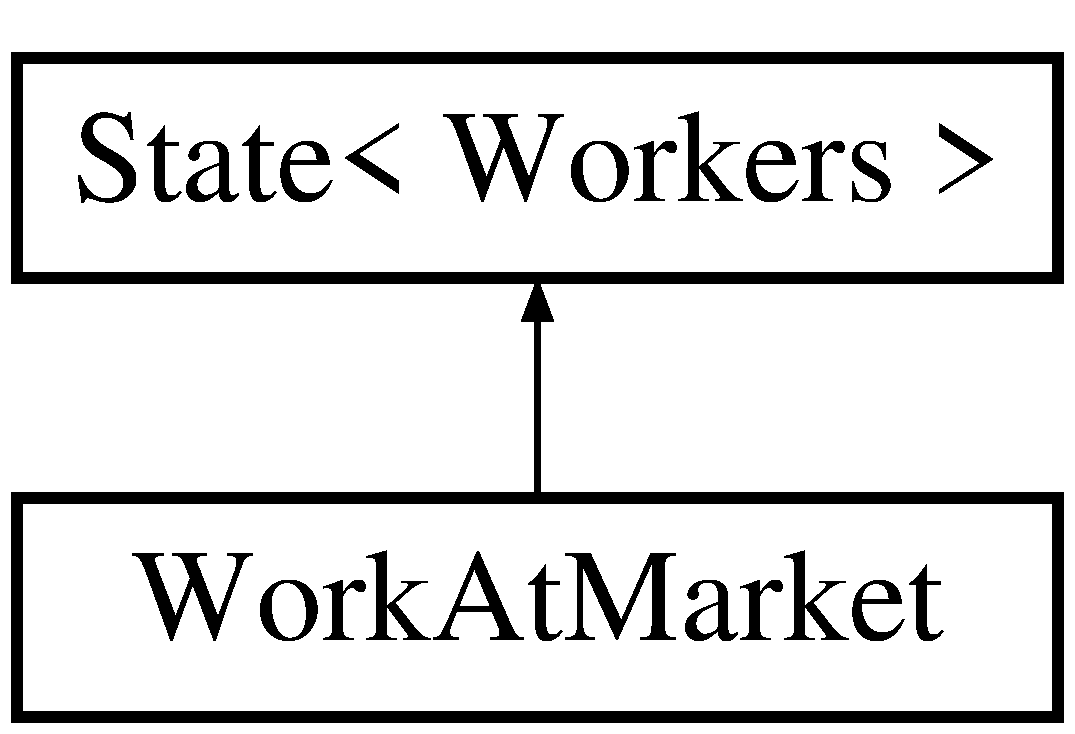
\includegraphics[height=2.000000cm]{class_work_at_market}
\end{center}
\end{figure}
\subsection*{Public Member Functions}
\begin{DoxyCompactItemize}
\item 
\hypertarget{class_work_at_market_ada2ea7b0283b28379d45d98e35350abe}{}virtual void {\bfseries State\+Enter} (\hyperlink{class_workers}{Workers} $\ast$worker)\label{class_work_at_market_ada2ea7b0283b28379d45d98e35350abe}

\item 
\hypertarget{class_work_at_market_a39ef36aad1d1808a2ff86a40fd27a21d}{}virtual void {\bfseries Execute} (\hyperlink{class_workers}{Workers} $\ast$worker)\label{class_work_at_market_a39ef36aad1d1808a2ff86a40fd27a21d}

\item 
\hypertarget{class_work_at_market_a6ea79e0610c166f4c8bd5facccdf404e}{}virtual void {\bfseries State\+Exit} (\hyperlink{class_workers}{Workers} $\ast$worker)\label{class_work_at_market_a6ea79e0610c166f4c8bd5facccdf404e}

\item 
\hypertarget{class_work_at_market_ab63b3ad172773e7cbd1323c063760cac}{}bool {\bfseries On\+Message} (\hyperlink{class_workers}{Workers} $\ast$worker, const \hyperlink{struct_telegram}{Telegram} \&msg)\label{class_work_at_market_ab63b3ad172773e7cbd1323c063760cac}

\end{DoxyCompactItemize}
\subsection*{Static Public Member Functions}
\begin{DoxyCompactItemize}
\item 
\hypertarget{class_work_at_market_a29eee057b4337047c6792f1a0b7e06ab}{}static \hyperlink{class_work_at_market}{Work\+At\+Market} $\ast$ {\bfseries Instance} ()\label{class_work_at_market_a29eee057b4337047c6792f1a0b7e06ab}

\end{DoxyCompactItemize}


The documentation for this class was generated from the following files\+:\begin{DoxyCompactItemize}
\item 
Labb1a/Entity\+States.\+h\item 
Labb1a/Entity\+States.\+cpp\end{DoxyCompactItemize}

\hypertarget{class_workers}{}\section{Workers Class Reference}
\label{class_workers}\index{Workers@{Workers}}
Inheritance diagram for Workers\+:\begin{figure}[H]
\begin{center}
\leavevmode
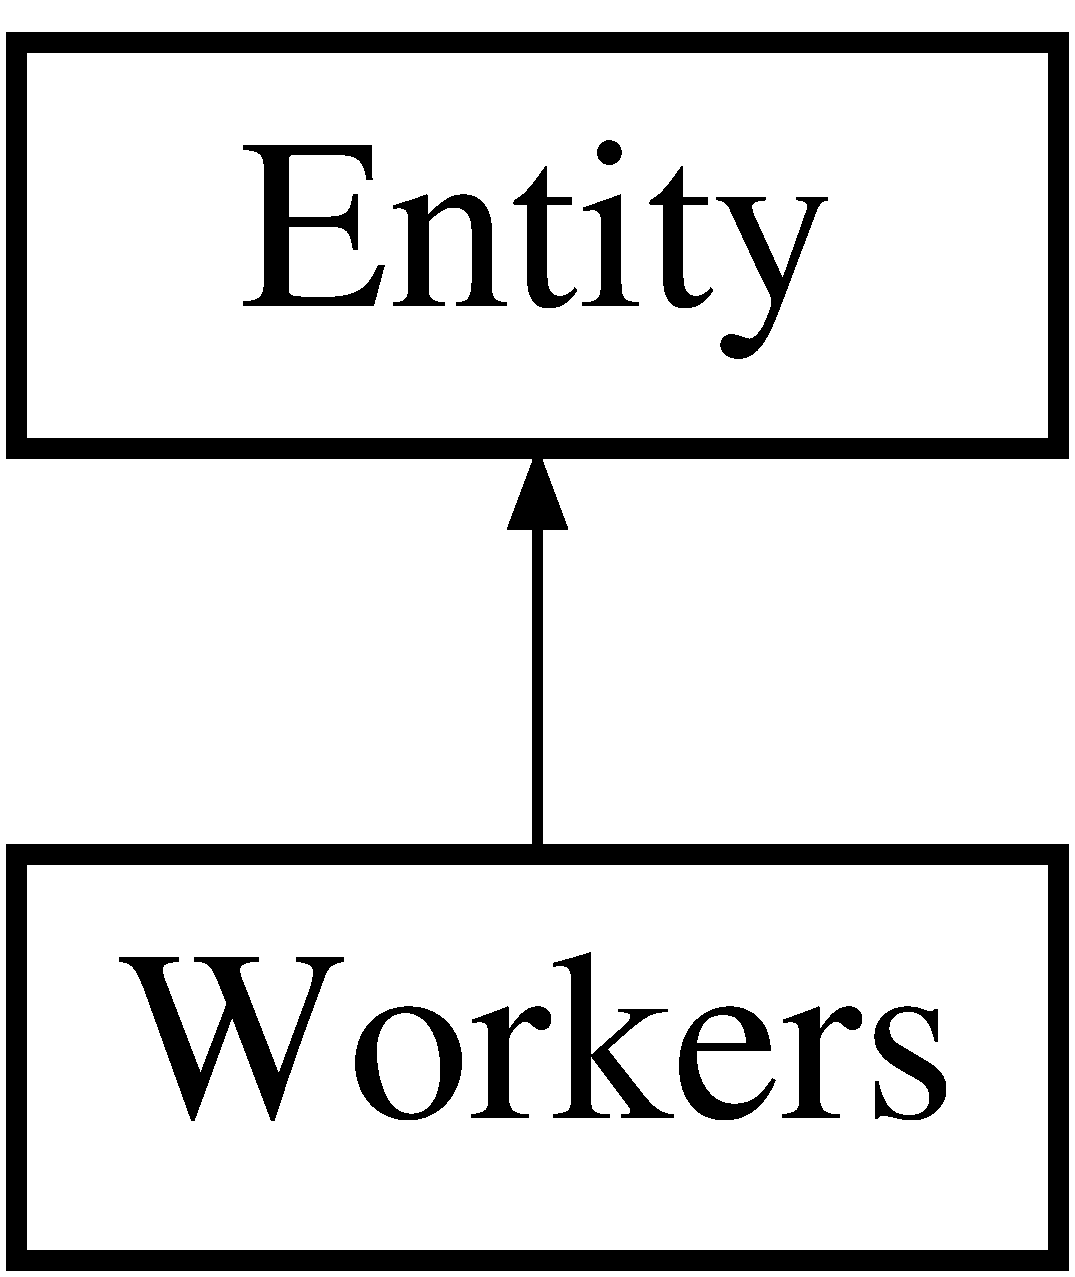
\includegraphics[height=2.000000cm]{class_workers}
\end{center}
\end{figure}
\subsection*{Public Member Functions}
\begin{DoxyCompactItemize}
\item 
\hypertarget{class_workers_aa90574d348fd6d9bce7aa4668c802f05}{}{\bfseries Workers} (int id)\label{class_workers_aa90574d348fd6d9bce7aa4668c802f05}

\item 
\hypertarget{class_workers_a70323696a9ef036f25978c0e7594bf3c}{}void {\bfseries Update} ()\label{class_workers_a70323696a9ef036f25978c0e7594bf3c}

\item 
\hypertarget{class_workers_a0ff295a940141b4b1b26cb483f4d5260}{}void {\bfseries Change\+Location} (location\+\_\+type l)\label{class_workers_a0ff295a940141b4b1b26cb483f4d5260}

\item 
\hypertarget{class_workers_a08857f839db217f4cc70270502cdc69c}{}location\+\_\+type {\bfseries get\+Location} ()\label{class_workers_a08857f839db217f4cc70270502cdc69c}

\item 
\hypertarget{class_workers_a2aaeb2392074ce8ea67bbe7469f378a5}{}void {\bfseries Add\+To\+Gold\+Carried} (const int val)\label{class_workers_a2aaeb2392074ce8ea67bbe7469f378a5}

\item 
\hypertarget{class_workers_ad4f6463e913c1d1d43cd724c3f3c0444}{}void {\bfseries Add\+To\+Wood\+Carried} (const int val)\label{class_workers_ad4f6463e913c1d1d43cd724c3f3c0444}

\item 
\hypertarget{class_workers_a9e23fa6bafb721f4903e96bf0ce86b9f}{}void {\bfseries Add\+To\+Fish\+Carried} (const int val)\label{class_workers_a9e23fa6bafb721f4903e96bf0ce86b9f}

\item 
\hypertarget{class_workers_a665001fb311f834e0c22933d3285bcc3}{}void {\bfseries Steal} ()\label{class_workers_a665001fb311f834e0c22933d3285bcc3}

\item 
\hypertarget{class_workers_a3280f043e03e520927d8bd3b468c7fc5}{}void {\bfseries Boost\+Morale} ()\label{class_workers_a3280f043e03e520927d8bd3b468c7fc5}

\item 
\hypertarget{class_workers_a83b50a9d70296590b9337c9c2f31c31c}{}bool {\bfseries Lonely} ()\label{class_workers_a83b50a9d70296590b9337c9c2f31c31c}

\item 
\hypertarget{class_workers_a580e6510e5bce327bf52752f5a5eede4}{}bool {\bfseries Depressed} ()\label{class_workers_a580e6510e5bce327bf52752f5a5eede4}

\item 
\hypertarget{class_workers_a86858b55a66ed50efd24df91ceac9865}{}bool {\bfseries Pockets\+Full} ()\label{class_workers_a86858b55a66ed50efd24df91ceac9865}

\item 
\hypertarget{class_workers_a4199dc7acb3f510d58ae3bcd97009d17}{}bool {\bfseries Is\+Tiered} ()\label{class_workers_a4199dc7acb3f510d58ae3bcd97009d17}

\item 
\hypertarget{class_workers_a1642198a0a8e95965a556316ef730548}{}void {\bfseries Increase\+Fatigue} ()\label{class_workers_a1642198a0a8e95965a556316ef730548}

\item 
\hypertarget{class_workers_a24a13054720d85803e579dcf20a055c8}{}void {\bfseries Decrease\+Fatigue} ()\label{class_workers_a24a13054720d85803e579dcf20a055c8}

\item 
\hypertarget{class_workers_aa6f1cffaa81ff10ac2fbd84475dafe7a}{}bool {\bfseries rested} ()\label{class_workers_aa6f1cffaa81ff10ac2fbd84475dafe7a}

\item 
\hypertarget{class_workers_a5bfeee07357cbff1223da9cf8335509d}{}bool {\bfseries Is\+Thirsty} ()\label{class_workers_a5bfeee07357cbff1223da9cf8335509d}

\item 
\hypertarget{class_workers_a87829202ef7808f0d3463a558e3e7e96}{}void {\bfseries Drink} ()\label{class_workers_a87829202ef7808f0d3463a558e3e7e96}

\item 
\hypertarget{class_workers_ab0aacaf426d3f23670b4f660fac72edc}{}bool {\bfseries Hungry} ()\label{class_workers_ab0aacaf426d3f23670b4f660fac72edc}

\item 
\hypertarget{class_workers_aaac02fee0fb8515edff148f07b16ae97}{}void {\bfseries Eat\+At\+Bar} ()\label{class_workers_aaac02fee0fb8515edff148f07b16ae97}

\item 
\hypertarget{class_workers_a352463eaf78a75a4116c3896c91e68b7}{}void {\bfseries Sell\+Goods} ()\label{class_workers_a352463eaf78a75a4116c3896c91e68b7}

\item 
\hypertarget{class_workers_ae479e00648b156fd50016c1e20930042}{}void {\bfseries Buy\+Stuff} ()\label{class_workers_ae479e00648b156fd50016c1e20930042}

\item 
\hypertarget{class_workers_a795643f5e05c591d4172f212ec77da90}{}\hyperlink{class_state_machine}{State\+Machine}$<$ \hyperlink{class_workers}{Workers} $>$ $\ast$ {\bfseries get\+State\+Machine} () const \label{class_workers_a795643f5e05c591d4172f212ec77da90}

\item 
\hypertarget{class_workers_a08cdcac34f5d3225b5faa5276ddc46ef}{}void {\bfseries set\+State\+Machine} (\hyperlink{class_state_machine}{State\+Machine}$<$ \hyperlink{class_workers}{Workers} $>$ $\ast$val)\label{class_workers_a08cdcac34f5d3225b5faa5276ddc46ef}

\item 
\hypertarget{class_workers_ae524c2a46d4c48ad5efcde956af6efe9}{}virtual bool {\bfseries Handle\+Message} (const \hyperlink{struct_telegram}{Telegram} \&msg)\label{class_workers_ae524c2a46d4c48ad5efcde956af6efe9}

\item 
\hypertarget{class_workers_aa0c46bd565afdb6652cf2f16b4ee221d}{}int {\bfseries get\+Fatigue} () const \label{class_workers_aa0c46bd565afdb6652cf2f16b4ee221d}

\item 
\hypertarget{class_workers_abb20740ab6c10e755c2a26896ec989a7}{}void {\bfseries set\+Fatigue} (int val)\label{class_workers_abb20740ab6c10e755c2a26896ec989a7}

\item 
\hypertarget{class_workers_a8f583ae979d5fd3dd80e5c59cd73d090}{}int {\bfseries get\+Currency} () const \label{class_workers_a8f583ae979d5fd3dd80e5c59cd73d090}

\item 
\hypertarget{class_workers_ac13a6bea46802080e06c0882382516dd}{}int {\bfseries get\+Wood} () const \label{class_workers_ac13a6bea46802080e06c0882382516dd}

\item 
\hypertarget{class_workers_a06bcad061d17843b5fb5728ee66ab175}{}void {\bfseries set\+Wood} (int val)\label{class_workers_a06bcad061d17843b5fb5728ee66ab175}

\item 
\hypertarget{class_workers_a7fdce044f9736c88cf0831c9efa9db5b}{}int {\bfseries get\+Fish} () const \label{class_workers_a7fdce044f9736c88cf0831c9efa9db5b}

\item 
\hypertarget{class_workers_a6ae83f7822640cda647414f1cd366b0c}{}void {\bfseries set\+Fish} (int val)\label{class_workers_a6ae83f7822640cda647414f1cd366b0c}

\item 
\hypertarget{class_workers_ad78c8b7ad9e6ea6ba3e8390eb5dc6498}{}int {\bfseries get\+Gold} () const \label{class_workers_ad78c8b7ad9e6ea6ba3e8390eb5dc6498}

\item 
\hypertarget{class_workers_a262c75ba2323327078ce2637d28d038a}{}void {\bfseries set\+Gold} (int val)\label{class_workers_a262c75ba2323327078ce2637d28d038a}

\item 
\hypertarget{class_workers_ae429543b8429ea7c52245e3c064c13ae}{}int {\bfseries get\+Hunger} () const \label{class_workers_ae429543b8429ea7c52245e3c064c13ae}

\item 
\hypertarget{class_workers_a2cd4cda944d4bf866a84940a35d598d8}{}void {\bfseries set\+Hunger} (int val)\label{class_workers_a2cd4cda944d4bf866a84940a35d598d8}

\item 
\hypertarget{class_workers_ad38a7b221ccbc9a705d4b14456ed5349}{}void {\bfseries set\+Thirst} (int val)\label{class_workers_ad38a7b221ccbc9a705d4b14456ed5349}

\item 
\hypertarget{class_workers_a2433e1d05f859980b8e37e64387d40ad}{}int {\bfseries get\+Thirst} () const \label{class_workers_a2433e1d05f859980b8e37e64387d40ad}

\item 
\hypertarget{class_workers_ae5dda4a3ee4766b4ecfce3b0485e1dda}{}void {\bfseries set\+Morale} (int val)\label{class_workers_ae5dda4a3ee4766b4ecfce3b0485e1dda}

\item 
\hypertarget{class_workers_aa1a129d2756bfa958916daf90e238f79}{}int {\bfseries get\+Morale} ()\label{class_workers_aa1a129d2756bfa958916daf90e238f79}

\item 
\hypertarget{class_workers_a95f49aa88ac7ee4db593e67ecd6093b9}{}void {\bfseries set\+Location} (location\+\_\+type val)\label{class_workers_a95f49aa88ac7ee4db593e67ecd6093b9}

\end{DoxyCompactItemize}


The documentation for this class was generated from the following files\+:\begin{DoxyCompactItemize}
\item 
Labb1a/Workers.\+h\item 
Labb1a/Workers.\+cpp\end{DoxyCompactItemize}

%--- End generated contents ---

% Index
\backmatter
\newpage
\phantomsection
\clearemptydoublepage
\addcontentsline{toc}{chapter}{Index}
\printindex

\end{document}
